\begin{table}[htbp]\small
\caption{Primary executed service resources. Includes production, independent verification and packaging; shared retrieval is reported separately.}
\begin{tabularx}{\linewidth}{@{}Yrrr@{}}
\toprule Arm & Accepted / planned & Total CPU s & CPU s / accepted\\ \midrule
A: Retained conventional & 3 / 6 & 1.274743 & 0.424914 \\
B: Workbench full & 3 / 6 & 4.658206 & 1.552735 \\
C: Incremental registry & 3 / 6 & 5.304753 & 1.768251 \\
D: Incremental graph & 3 / 6 & 4.863663 & 1.621221 \\
\bottomrule\end{tabularx}
\end{table}

The complete primary campaign used 16.139765 CPU seconds and
15.012749 elapsed seconds. Its driver overhead was
0.038400 CPU seconds, allocated separately from the table.
The all-input acquisition session used 4.806423 CPU seconds and 7.387453 elapsed seconds.
Source availability, normalized bytes, licenses and failed URLs are preserved in the input manifest.


\begin{figure}[htbp]\centering
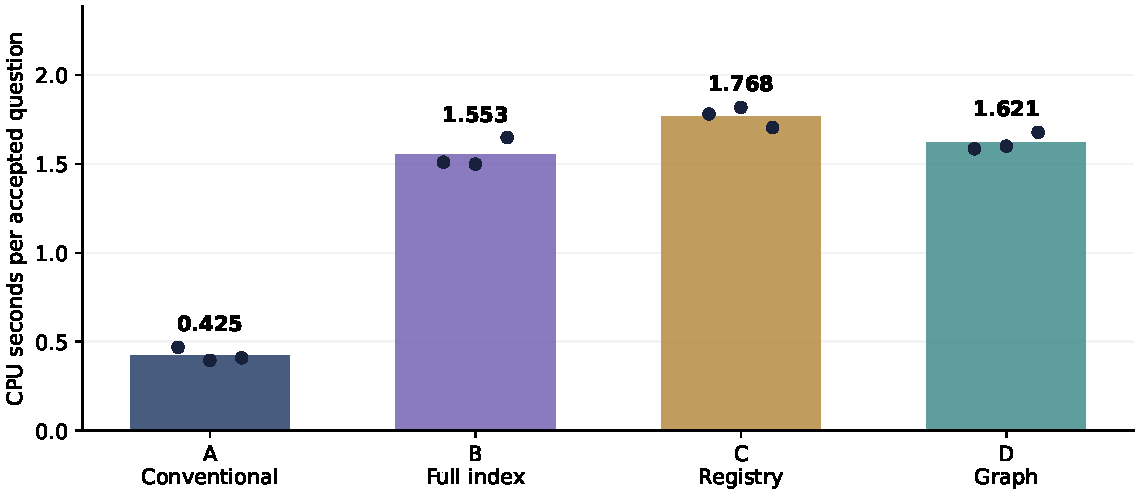
\includegraphics[width=0.9\linewidth]{figures/primary-cpu.pdf}
\caption{Each dot is one accepted primary question; bars are their mean. Complete compared delivery
includes independent verification and packaging. Three blocked questions per arm remain in the
intent-to-deliver denominator but do not become zero-duration successful jobs. One pass per case
does not establish a latency distribution. Shared acquisition and research costs are separate.}
\end{figure}

All four arms agree on the exact changed fact tuples and source provenance. The conventional
builder is faster in every available primary question. Incremental reuse does not improve the
primary average over the full Workbench index. The graph mean is slightly below the registry mean
in this single run, but it creates no additional accepted work and supplies no independently
identified planning advantage. Both remain slower than the conventional builder.

The public-tool supplement strengthens the alternative. After validated Swagger2-to-OpenAPI
conversion, oasdiff 1.34.1 reports 102, 5 and 0 breaking findings and 365, 9 and 77 changelog
items on the three available pairs. Its broader request/response/media coverage is not the same
acceptance task as the structural dossier. Raw Swagger2 supplied to the OpenAPI3 validation contract produced 15, 1 and 0
findings despite 103--105 validation errors; default exit zero therefore did not establish a
valid result. A YAML parser failure on v20 was preserved, then a separately labeled follow-up
used the existing frozen normalized JSON. All 27 supplemental commands, including invalid and
failed attempts, used 6.280 seconds wall and 8.923 CPU seconds. No primary producer was rerun.
